\documentclass[compress,10pt,aspectratio=169]{beamer}
%\setbeamertemplate{background canvas}[bottom=white,top=structure.fg!25]
%\usetheme{Hannover}
\setbeamertemplate{headline}{}
\setbeamertemplate{footline}{June 27, 2020 - SDRA}
\setbeamersize{text margin left=0.1cm}
\usepackage{appendixnumberbeamer,fancyvrb}
\usepackage{hyperref,listings,picinpar,mathtools} % ,enumitem}
\usepackage{color}
\settowidth{\leftmargini}{\usebeamertemplate{itemize item}}
\addtolength{\leftmargini}{\labelsep}
\usepackage{fancyvrb}
\usepackage{xcolor}

\definecolor{grey}{rgb}{0.95,0.95,0.95}
\definecolor{red}{rgb}{1.0,0.0,0.0}
\definecolor{green}{rgb}{0.0,0.6,0.0}
\definecolor{blue}{rgb}{0.0,0.0,1.0}
\lstloadlanguages{bash,Java,C,C++,csh,make,sh}%%[Visual]Basic,xml}
\lstset{frame=none,basicstyle=\tiny,breaklines,tabsize=2,captionpos=b,prebreak={\hbox{$\rightarrow$}},postbreak={\hbox{$\hookrightarrow$}},showstringspaces=false,backgroundcolor=\color{grey}\bfseries,keywordstyle=\color{blue},commentstyle=\color{green}\textit,stringstyle=\color{red}\ttfamily,abovecaptionskip=2pt,aboveskip=0pt,belowskip=0pt,belowcaptionskip=0pt}
%\lstset{moredelim=[is][\color{red}]{_+_}{_+_}}

\beamertemplatefootpagenumber
\beamertemplatenavigationsymbolsempty
\setbeamertemplate{footline}[page number]{}
\setbeamertemplate{page number in head/foot}{}

\usepackage{graphicx,verbatim,multicol,amsmath,bm}
\graphicspath{{./figures/}{../pictures/}}

\begin{document}
\title{Yet Another White Rabbit running on a low-cost, generic FPGA board}
\author{\'Emilien Decoux, Jean-Michel Friedt\\ \ \\ 
FEMTO-ST Time \& Frequency department, Besan\c con, France \\ \ 
\\ \ \\ jmfriedt@femto-st.fr \ \\ \ \\
project archive at \url{https://github.com/oscimp/wr_acorn}\\
%\vspace{-1.27cm}
\parbox{1.0\linewidth}{\includegraphics[width=.3\linewidth]{logo_femto.pdf}\hfill
%\includegraphics[width=.37\linewidth]{gnuradio_logo.pdf}
}\vspace{-1cm}  
}
\maketitle

\begin{frame}[fragile]\frametitle{Context and outline}

\begin{minipage}[t]{\linewidth}
\begin{minipage}{.49\linewidth}    
{\footnotesize
\begin{itemize}
\item White Rabbit (WR) supported boards require two dedicated oscillators for generating
the digital phase detector (DMTD)
\item WR as feature of generic boards (RF signal acquisition and synthesis, Software Defined Radio -- SDR) requires getting rid of this requirement
\item Use of clocking circuits internal to the FPGA for generating WR clocks
\item Demonstration on Enjoy Digital's Acorn CLE215+ board...
\item ... Xilinx Artix-7 A100T FPGA / 1 Gb DDR $\Rightarrow$ start from Nikhef's  CLBv3 design and Missing Link Electronics' 2024 contribution\footnotemark
\footnotemark
\end{itemize}
}
\end{minipage}
\begin{minipage}{.49\linewidth}
\includegraphics[width=\linewidth]{IMG_20250425_163316_728.jpg}
\end{minipage}
\end{minipage}
\footnotetext{\url{https://enjoy-digital-shop.myshopify.com/products/litex-acorn-baseboard-mini-sqrl-acorn-cle215} 215 euros + SFP adapters}
\footnotetext{13th White Rabbit Workshop (CERN), \url{https://www.missinglinkelectronics.com/wp-content/uploads/2024/03/MLE-Light-Rabbit-Presentation-at-13th-White-Rabbit-Workshop.pdf}}
\end{frame}

\begin{frame}[fragile]\frametitle{VCO-less DMTD implementation and characterization}
\end{frame}

\begin{frame}[fragile]\frametitle{HDL implementation on CLE215+}

  \begin{itemize}
    \item \texttt{board/acorn/} - FPGA-internal HDL
      \begin{itemize}
        \item \texttt{Manifest.py} - hdlmake imports
        \item \texttt{wr\_acorn\_pkg.vhd} - hdl header
        \item \texttt{xwrc\_board\_acorn.vhd} - logic around \texttt{xwrc\_platform\_xilinx} and \texttt{xwrc\_board\_common}
          \begin{itemize}
            \item \texttt{xwrc\_board\_common} expose dac interfaces outputs and clock inputs
            \item traditionnal WR convert \texttt{data+load} to I²C/other dac protocol
            \item VCO-less WR convert \texttt{data+load} to MMCM's phase-shift control
          \end{itemize}
      \end{itemize}
    \item \texttt{top/acorn\_ref\_design/} - FPGA/board interface files

          \texttt{acorn\_wr\_ref\_top.xdc} - set io pins and allow internal clocking of the GTP ports
    \item \texttt{syn/acorn\_ref\_design/} - synthesis related files
          add custom \texttt{bitstream.tcl} to allow internal clocking of the GTP ports
    \item \texttt{platform/Xilinx} - add generic to allow internal clocking of the GTP ports
  \end{itemize}

\end{frame}


\begin{frame}[fragile]\frametitle{LiteX implementation on CLE215+: {\footnotesize\url{https://github.com/enjoy-digital/litex_wr_nic}}}

{\scriptsize
\begin{verbatim}
wrc# pll stat
softpll: mode:3 seq:ready n_ref 1 n_out 1
irqs:123226 alignment_state:0 HL1 ML1 HY=23493 MY=40133 DelCnt=0 setpoint:13037 refcnt:66565 tagcnt:53
softpll: ptracker0: enabled 1 n_avg 512 value 13575
wrc# gui
SPA7 WRPC Monitor wrpc-v5.0-ohwr-9-g5ac04dd5-dirt | Esc/q = exit; r = redraw

TAI Time: 2023-03-03-11:55:43  UTC offset: 37   PLL mode: BC  state: Locked
---+-------------------+-------------------------+---------+---------+-----
 # |        MAC        |       IP (source)       |    RX   |    TX   | VLAN
---+-------------------+-------------------------+---------+---------+-----
 0 | 22:33:44:55:66:77 |                         |     555 |     183 |    0
--- HAL ---|------------- PPSI ------------------------------------------------
 Itf | Frq |  Config   | MAC of peer port  |    PTP/EXT/PDETECT States   | Pro 
-----+-----+-----------+-------------------+-----------------------------+-----
 wr0 | Lck | auto      | 70:b3:d5:91:ea:f0 | SLAVE    /IDLE      /EXT_ON | R-W 
Pro(tocol): R-RawEth, V-VLAN, U-UDP

--------------------------- Synchronization status ----------------------------
Servo state:          White-Rabbit: TRACK_PHASE                         

--- Timing parameters ---------------------------------------------------------
meanDelay        :              284.572 ns
delayMS          :              284.572 ns 
delayMM          :             1097.210 ns 
delayAsymmetry   :                0.000 ns
delayCoefficient :   +0.000000000000000000  fpa   0
...
\end{verbatim}
}
\end{frame}

\begin{frame}[fragile]\frametitle{Results: Acorn CLE215+}

Tuning software phase locked-loop (PLL) control coefficients

\begin{minipage}[t]{\linewidth}
\begin{minipage}{.49\linewidth}
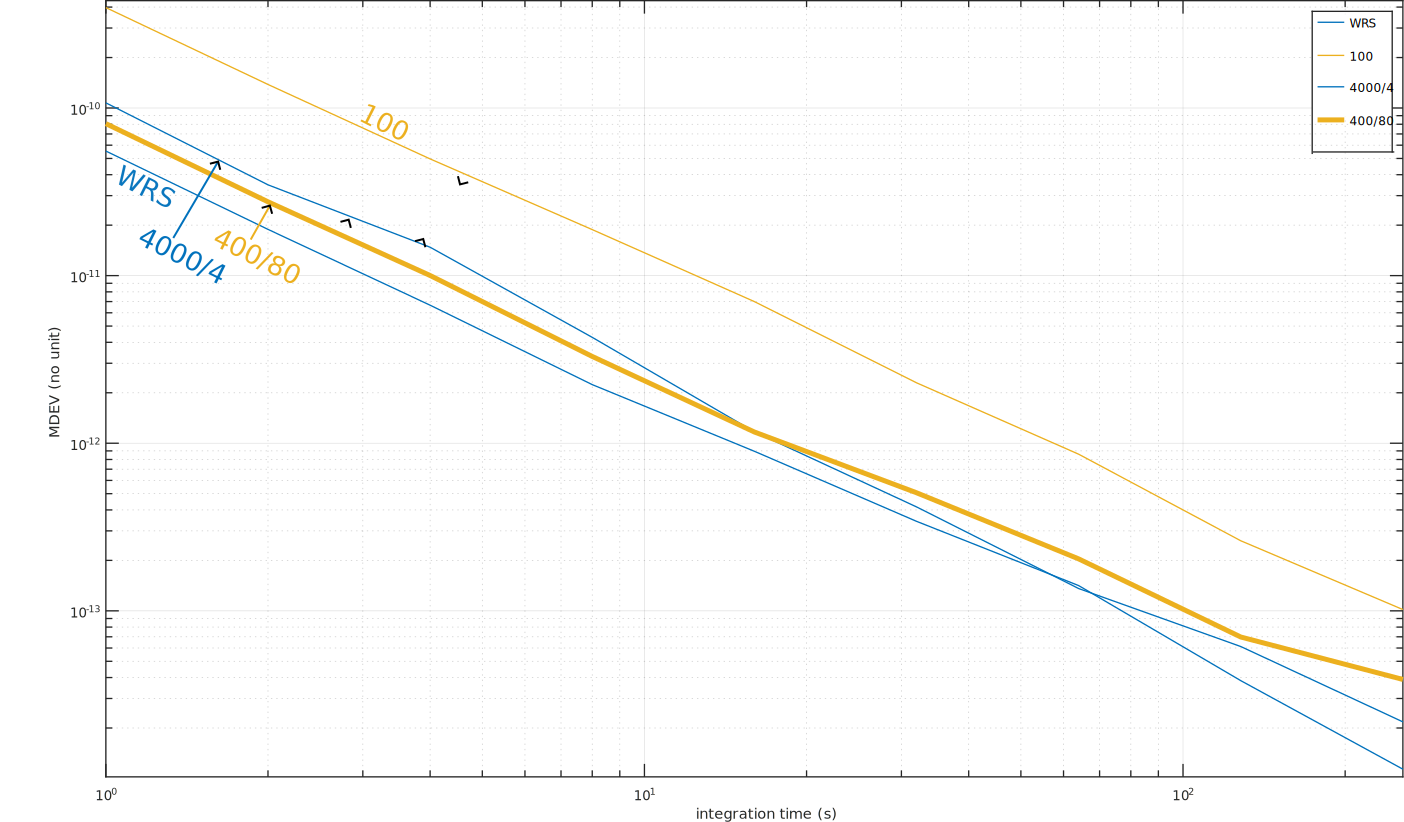
\includegraphics[width=\linewidth]{allan_wr_acorn_new.pdf}

Modified Allan deviation: phase flicker noise
\end{minipage}
\begin{minipage}{.49\linewidth}
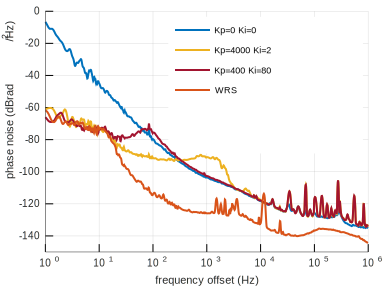
\includegraphics[width=\linewidth]{phase_noise_litex.pdf}

Phase noise (Rohde \& Schwarz FSWP, all 10~MHz except LiteX 62.5~MHz
scaled)
\end{minipage}
\end{minipage}

Low quality 200~MHz MEMS oscillator
\end{frame}

\begin{frame}[fragile]\frametitle{Results: M2SDR}

\begin{minipage}[t]{\linewidth}
\begin{minipage}{.49\linewidth}
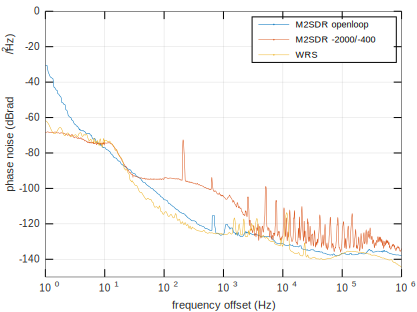
\includegraphics[width=\linewidth]{m2sdr.pdf}
\end{minipage}
\begin{minipage}{.49\linewidth}
\includegraphics[width=\linewidth]{M2SDR_vs_WRS_allan}
\end{minipage}
\end{minipage}

100~MHz TCXO oscillator
\end{frame}

\begin{frame}[fragile]\frametitle{Reference clock characteristics}

\begin{minipage}[t]{\linewidth}
\begin{minipage}{.49\linewidth}
\end{minipage}
\begin{minipage}{.49\linewidth}
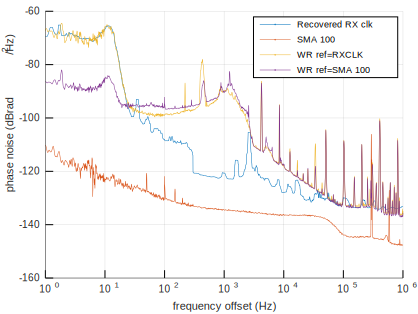
\includegraphics[width=\linewidth]{phase_noise.pdf}
\end{minipage}
\end{minipage}
\end{frame}

\begin{frame}[fragile]\frametitle{Phase detection characteristics}

\begin{minipage}[t]{\linewidth}
\begin{minipage}{.49\linewidth}
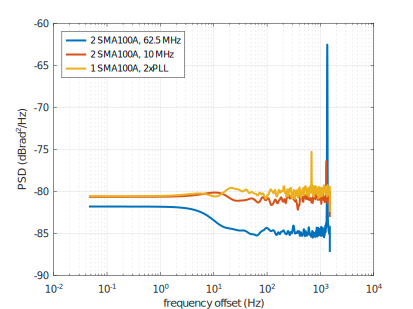
\includegraphics[width=\linewidth]{62p5MHz.pdf}
\end{minipage}
\begin{minipage}{.49\linewidth}
\end{minipage}
\end{minipage}
\end{frame}

\begin{frame}[fragile]\frametitle{Conclusion \& perspectives}

Acknowledgements: 
\begin{itemize}
    \item Peter Jansweijer (Nikhef) for updating the CLBv3 design, 
    \item Frederik Pfautsch (Missing Link Electronics) for committing the various VCO-less implementations, 
    \item Florent Kermarrec and Gwenhael Goavec-Merou (Enjoy Digital) for providing the
    hardware boards and LiteX implementations
    \item CERN's White Rabbit team (Tomasz Wlostowski, Tristan Gingold \& others) 
    \end{itemize}
\end{frame}
\end{document}
